\newpage
\subsection{Problems}


\begin{tcolorbox}
\noindent {\bf Problem \thesection.\theprob}\stepcounter{prob}

The revolution number of a water pump is 1470 rpm, the flow rate is $Q=0.055\mathrm{m^3/s}$ and the head is $H=45$m. The hydraulic power loss is $P'_h=2.5$kW, the mechanical power loss is $P'_m=1.3$kW, the disc friction coefficient is $\nu_t=0.065$. The input power at this operating point is $P_{in}=32$kW. Make a complete analysis of the losses, including leakage flow rate and the theoretical head.

\noindent Solution:

The power flow chart is in Figure \ref{gen_pfc}

\begin{itemize}
\item $P_{i}=P_{input}-P'_{m}=30.7\,\mathrm{kW}\quad \rightarrow \quad \eta_{m}=95.9\%$
\item $P_{th}=(1-\nu)P_{i}=28.7\,\mathrm{kW}$
\item $h'_{h}=\frac{P'_{h}}{\rho g Q}=4.63\,\mathrm{m} \quad \rightarrow \quad H_{th}=45+4.63=49.63\,\mathrm{m}\quad \rightarrow \quad \eta_{hydr}=90.6\%$
\item $Q_{th}=\frac{P_{th}}{\rho g H_{th}}=0.0589\,\mathrm{m^3/s}\quad \rightarrow \quad Q_{leakage}=0.00395\,\mathrm{m^3/s}\quad \rightarrow \quad \eta_{v}=93.2\%$ 
\item $\eta_{overall}=\eta_{v} \cdot\eta_{h} \cdot (1-\nu) \cdot \eta_{m} = 75.9\%$
\end{itemize}
\end{tcolorbox}
\vspace{1cm}

\begin{figure}[ht]
\begin{center}
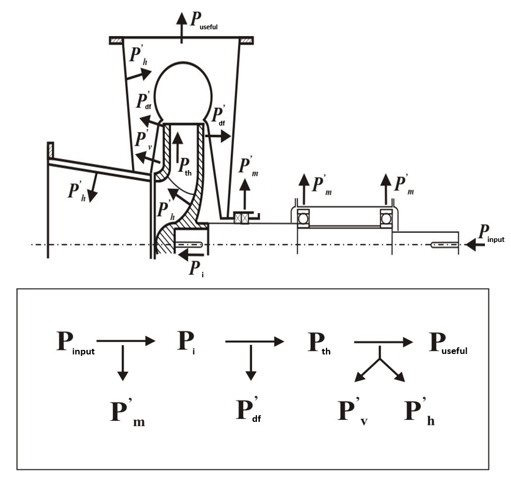
\includegraphics[scale=0.85]{figs/problem_2p3p17_pow_flow_chart_fig.png}
\caption{\label{gen_pfc}Power flow chart}
\end{center}
\end{figure}

\vspace{1cm}
\noindent {\bf Problem \thesection.\theprob}\stepcounter{prob}

\note{problem added by Weber Richard}
Calculate the theoretical head, the theoretical volume flow rate, the hydraulic efficiency and the volumetric efficiency based on the data of the water pump. $P_{input} = 43.5\,kW,$ $Q = 1100\,dm^3/min,$ $H = 180\,m,$ $P'_{mech} = 1.6\,kW,$ $\nu_{df} = 0.03, h' = 32\,m$.
(Solution: $H_{th} = 212\,m,$ $Q_{th} = 0.01954\,m^3/s$ $\eta_{hydr} = 84.9\%$ $ \eta_{vol} = 93.8\%$)